\chapter{Classification}
\begin{dfnbox}{Classification}{c}
    \hspace{2em}\dfntxt{Classification} is a process of categorizing a given set of data into classes. It can be performed on both structured or unstructured data. The process starts with predicting the class of given data points. The classes are often referred to as target, label or categories.
\end{dfnbox}

\begin{dfnbox}{Binary classification}{bc}
\hspace{2em}Binary or binomial classification is the task of classifying the elements of a given set into two groups on the basis of a classification rule. In binary classification, the output is a binary value, such as yes/no, 0/1, true/false, etc.
\tcblower
\hspace{2em}Usually, the two classes/categories are represented by 0 and 1.
we call the 0 as the negative class and the 1 as the positive class.
\end{dfnbox}

\section{Linear Regression approach to Classification}
we can use linear regression for classification problems, but it is not a good idea.\\
The problem with linear regression is that it tries to predict the output as a continuous value.\\
In the case of binary classification, the output is a binary value, 0 or 1.\\

\begin{exbox}{Linear Regression for Binary Classification}{}
    \hspace{2em}Let's say we have a binary classification problem with two classes, 0 and 1.
    We can use linear regression to predict the output.
    The output of linear regression can be any real number, which can be greater than 1 or less than 0.
    We can set a threshold value, say 0.5. If the output is greater than 0.5, we can classify it as 1, and if it is less than 0.5, we can classify it as 0.\par
    \hspace{2em}Take the example of predicting a tumor as malignant or benign.

    \begin{minipage}{0.5\textwidth}
        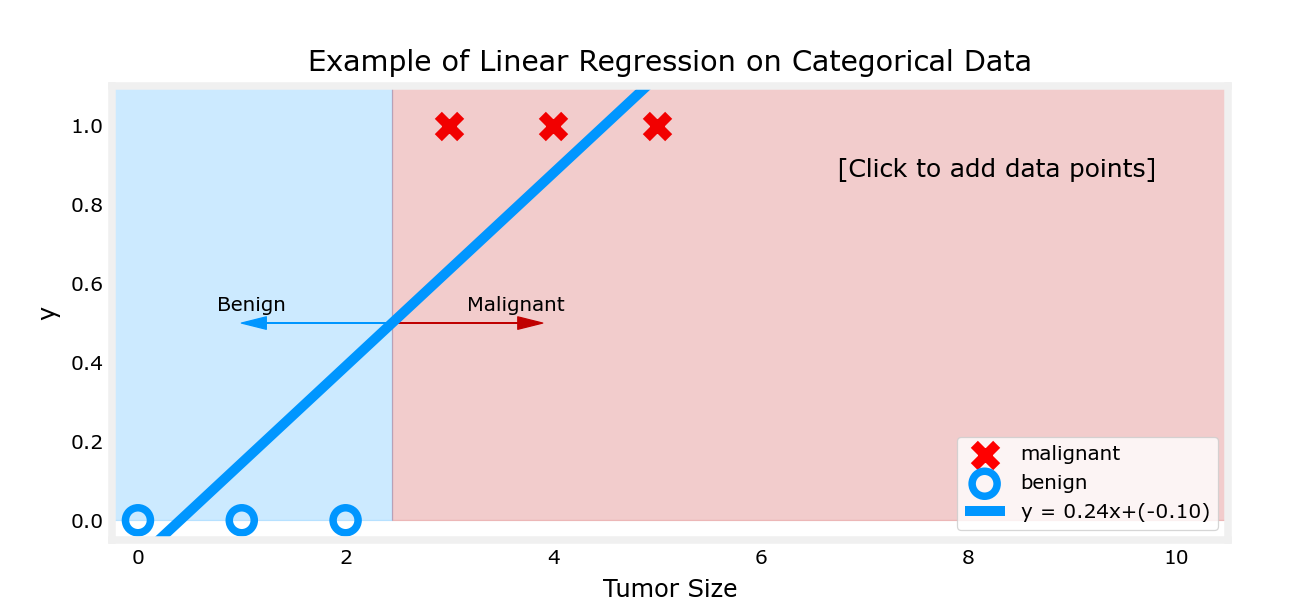
\includegraphics[width=\textwidth]{images/6.1.1.png}
    \end{minipage}
    \begin{minipage}{0.5\textwidth}
        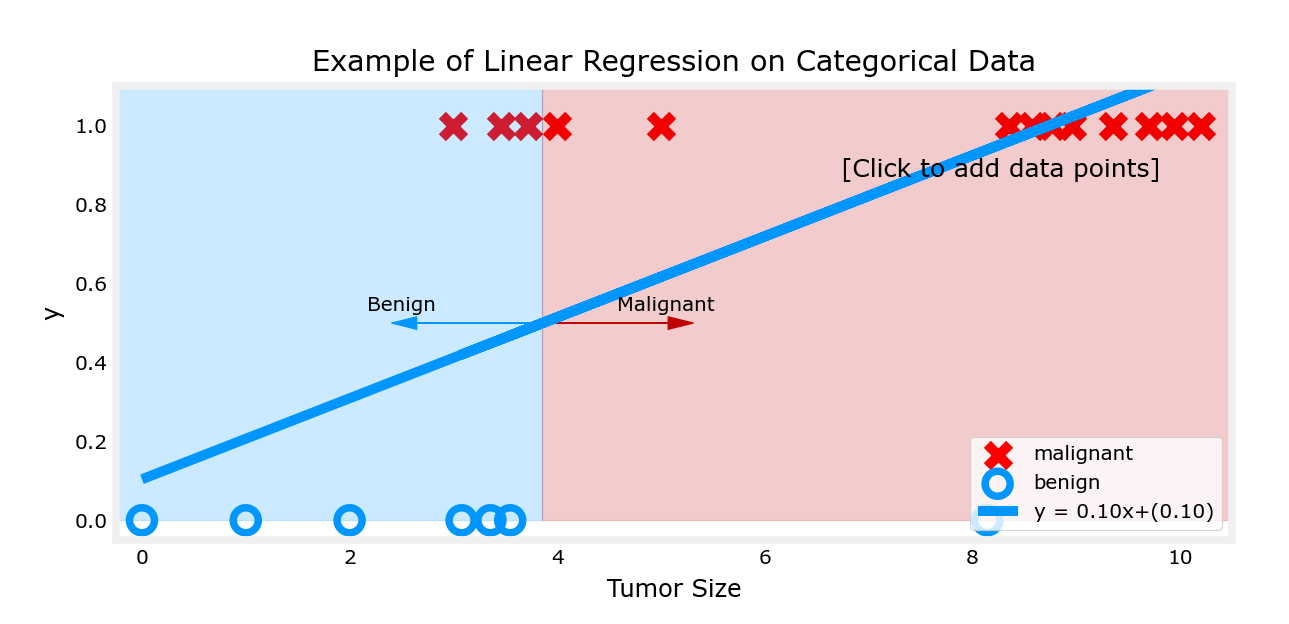
\includegraphics[width=\textwidth]{images/6.1.2.png}
    \end{minipage}

    \hspace{2em}In the above figure, if we add more malignant tumors with a large size, the line will shift towards the malignant side.
    This will cause the malignant tumors to be classified as benign.
    However, the malignant tumors are still malignant, but they are classified as benign because of the shift in the line.
\end{exbox}


\section{Logistic Regression}
\begin{dfnbox}{Logistic Regression}{lr}
    \hspace{2em}\dfntxt{Logistic regression} is a statistical model that in its basic form uses a logistic function
    to model a binary dependent variable.
    \begin{align}
        \mathrm{sigmoid\ function / logistic\ function:}& \nonumber\\
        g(z) = \frac{1}{1 + e^{-z}}& \qquad 0 < g(z) < 1
    \end{align}
    \centering
    \includegraphics*[width=0.8\textwidth]{images/Figure 4}
\end{dfnbox}

\begin{thmbox}{Logistic Regression}{lr}
    We can transform the output of linear regression using the sigmoid function.
    \begin{align*}
        f_{(\mathbf{w}, b)}(\mathbf{x}) &= g(z) \\
        z &= \mathbf{w}^T \mathbf{x} + b \\
        g(z) &= \frac{1}{1 + e^{-z}}\\
        & \ \Downarrow\\
        f_{(\mathbf{w}, b)}(\mathbf{x}) &= g(\mathbf{w}^T \mathbf{x} + b) = \frac{1}{1 + e^{-(\mathbf{w}^T \mathbf{x} + b)}}
    \end{align*}
\end{thmbox}

\paragraph*{Interpretation of the output}
The output of logistic regression is the probability that 
the given input point belongs to the positive class.(class 1)\\
\begin{equation}
    f_{(\mathbf{w}, b)}(\mathbf{x}) = P(y = 1 | \mathbf{x}; \mathbf{w}, b)
\end{equation}

\begin{notebox}
    \hspace{2em}By using the sigmoid function, the output of logistic regression is always between 0 and 1.
    And it provide a nonlinear fit curve, which solves the problem of linear regression in the previous tumor example.
    
    \centering
    \includegraphics*[width=0.8\textwidth]{images/6.1.3}
\end{notebox}

\section{Decision Boundary}
\paragraph*{How to classify?}
when the output of logistic regression is greater than 0.5,
we classify it as 1, and when it is less than 0.5, we classify it as 0.
\par
By looking at the sigmoid function,
 we can see that the output of logistic regression is greater than 0.5 when $z > 0$ and less than 0.5 when $z < 0$.
Which is to say when $\mathbf{w}^T \mathbf{x} + b > 0$,
 we classify it as 1, and when $\mathbf{w}^T \mathbf{x} + b < 0$, we classify it as 0.\\

\begin{notebox}
    \hspace{2em}The decision boundary is the line that separates the positive class from the negative class.
    It is the line where $z=0$. In the function diagram, we can draw the image of the function $z=0$. For example,
    if we have two features $x_1$ and $x_2$, the decision boundary is the line where $w_1 x_1 + w_2 x_2 + b = 0$.
    and the $z$ can be also other comlex functions. Such as $z = w_1 x_1^2 + w_2 x_2^2 + b$, which is a circle.
\end{notebox}

\begin{center}
    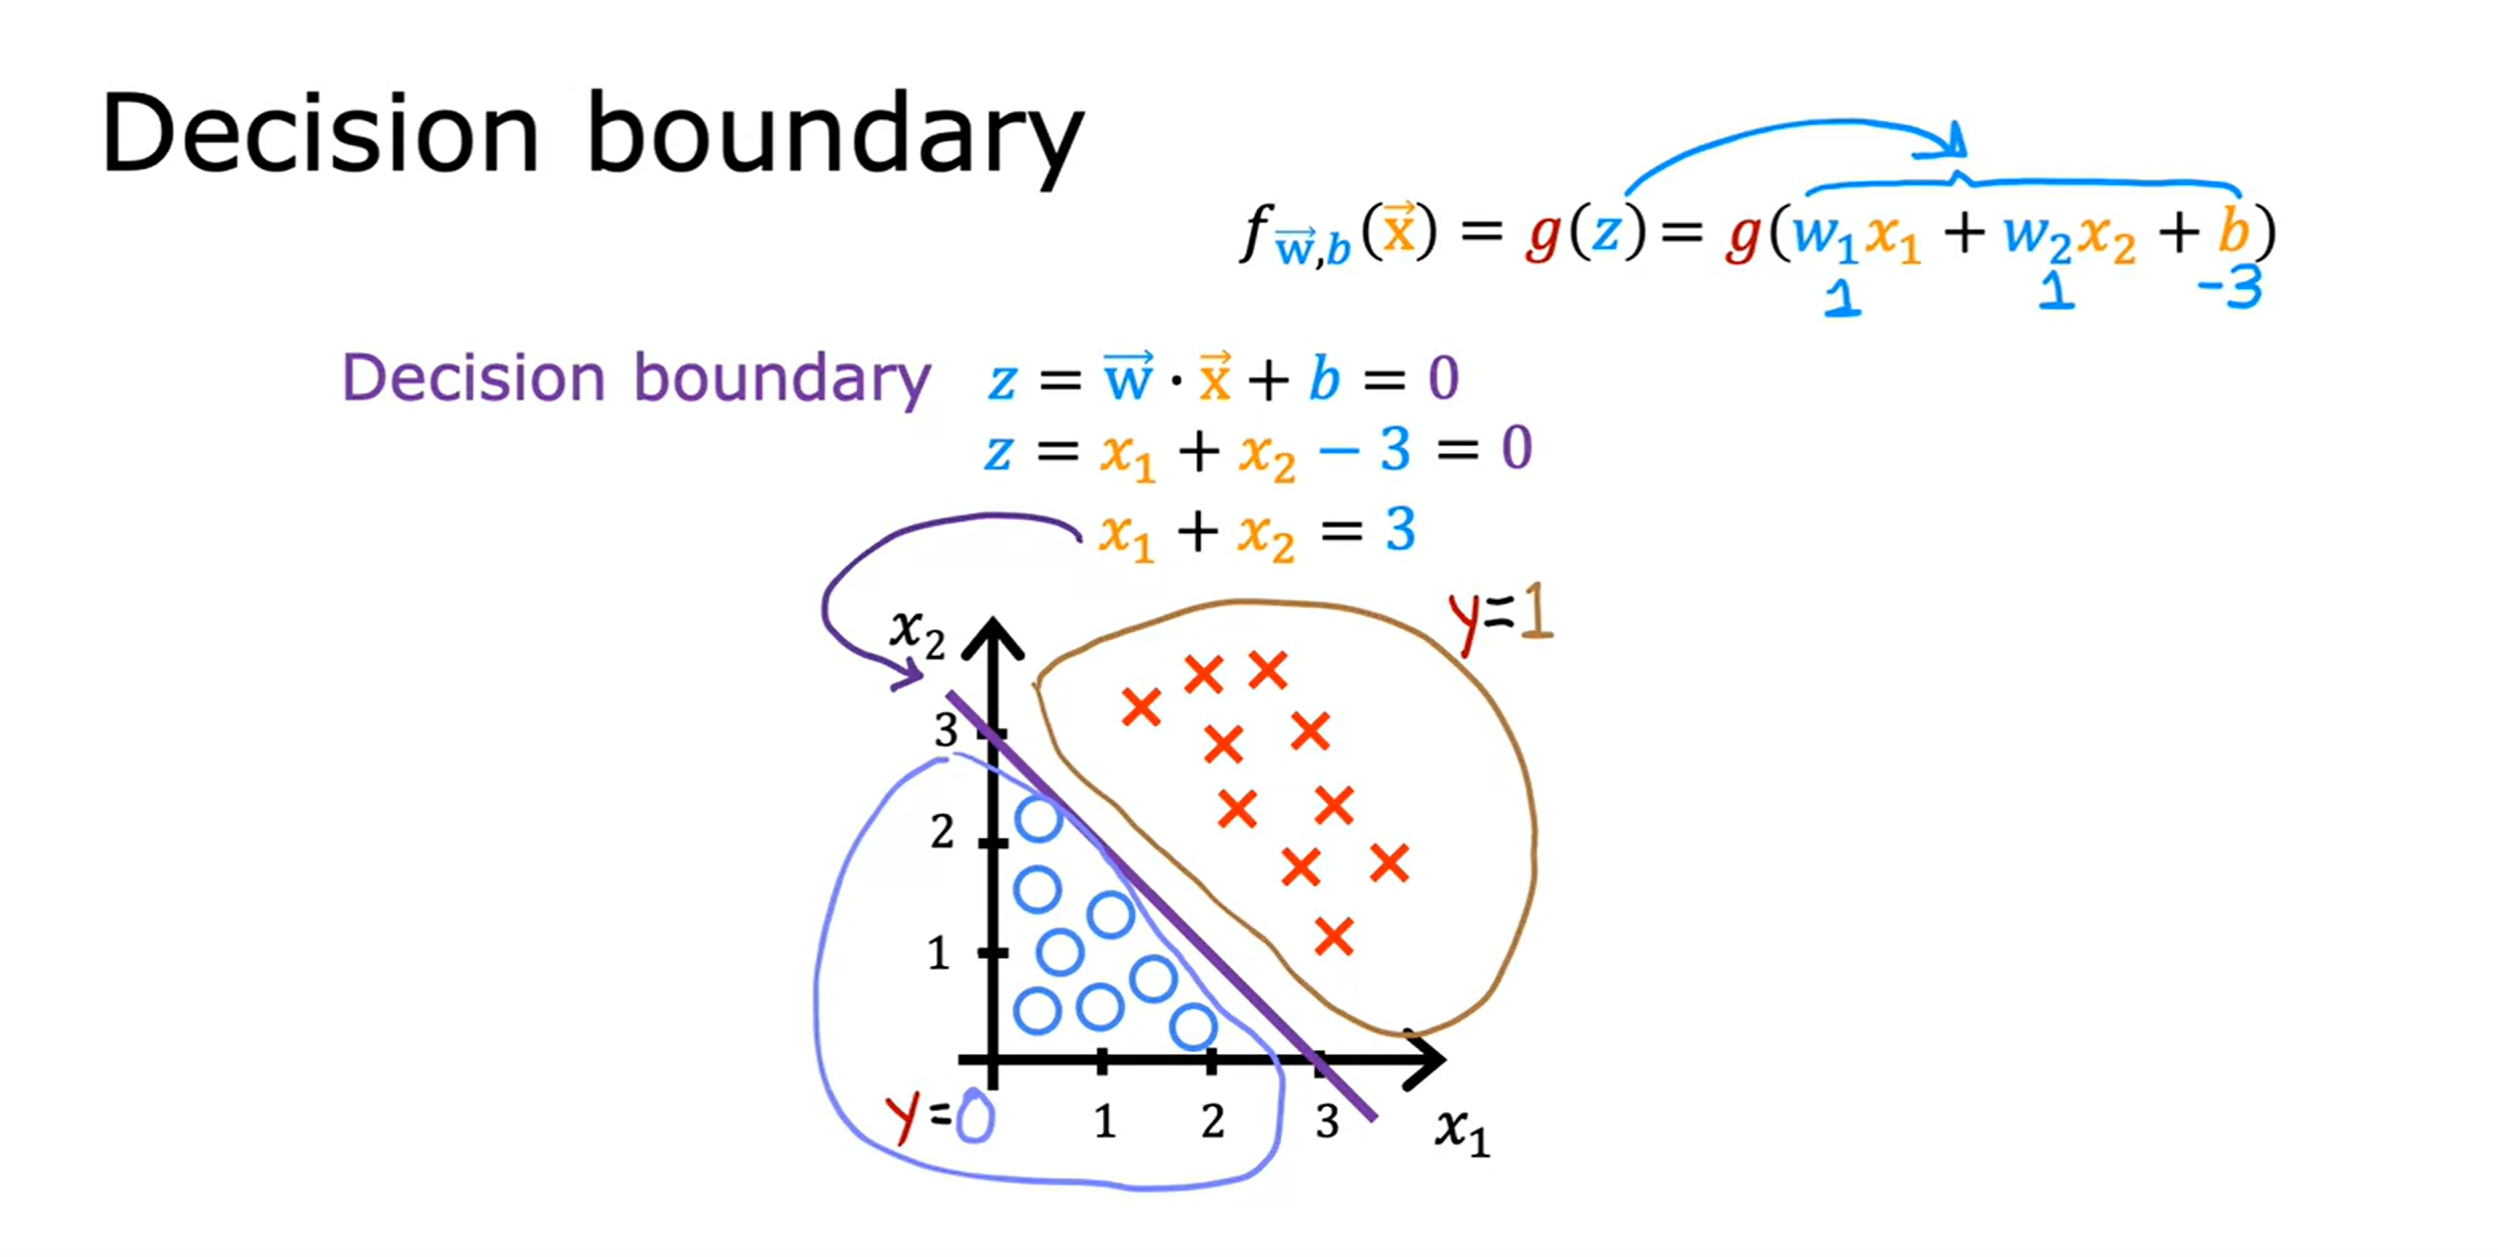
\includegraphics[width=0.7\textwidth]{images/6.1_3 (2)}\\
    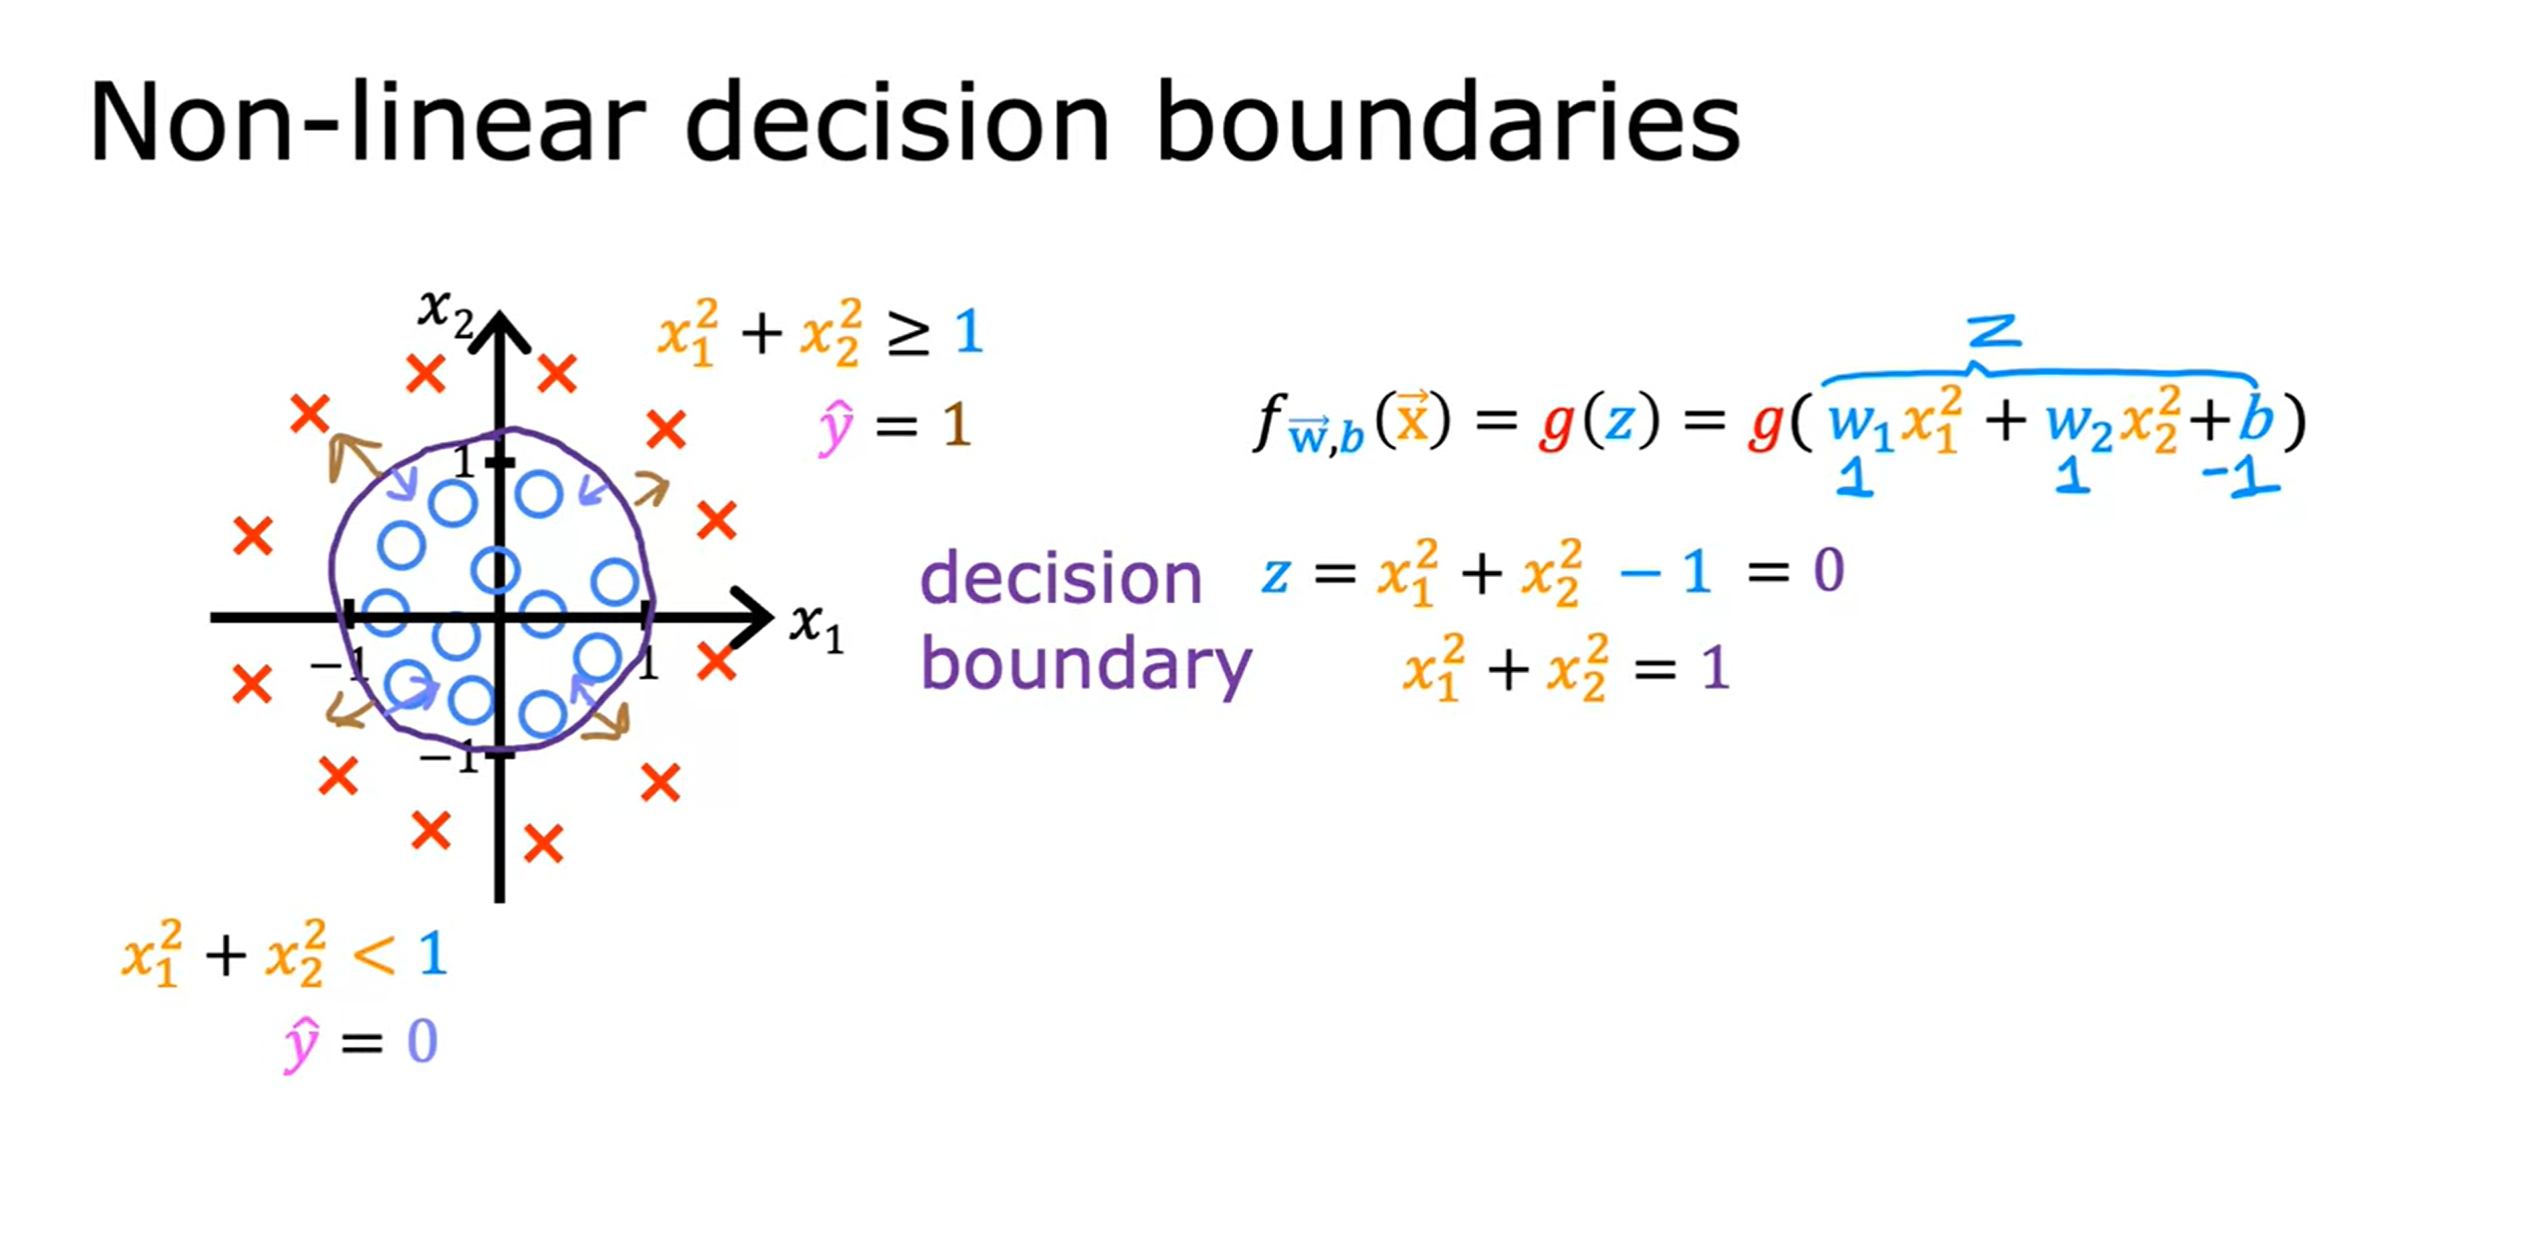
\includegraphics[width=0.7\textwidth]{images/6.1_3 (1)}\\
    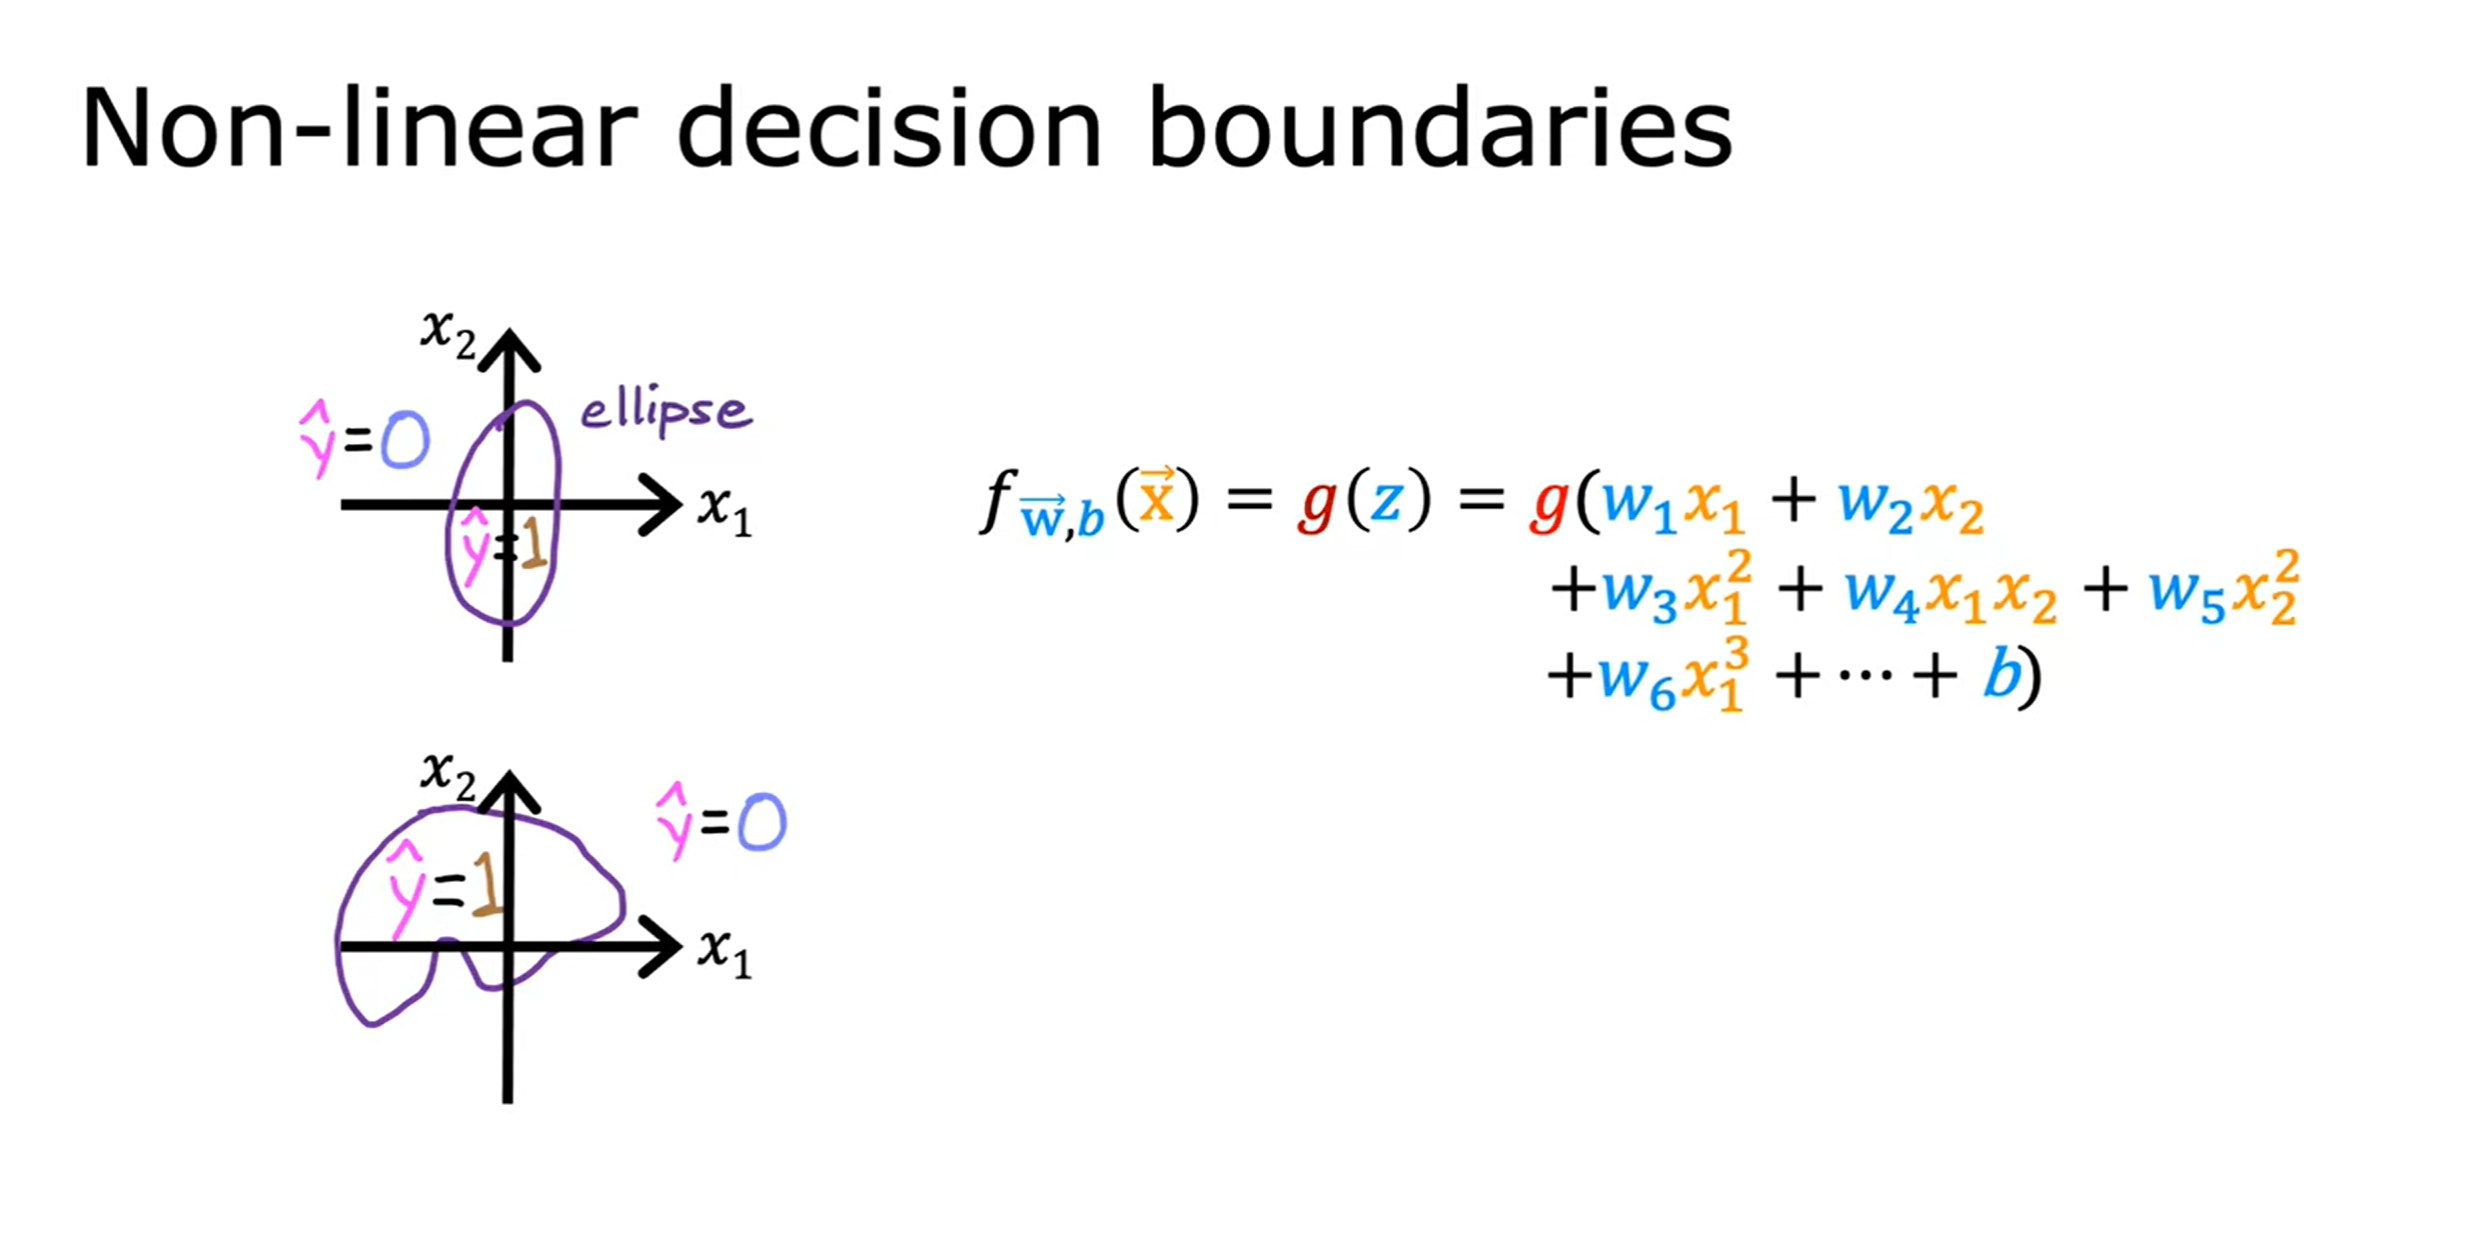
\includegraphics[width=0.7\textwidth]{images/6.1_3 (3)}
\end{center}
 
\section{Cost Function}
\paragraph*{Why it is unreasonable to use the cost function of linear regression?}\leavevmode

The squared error cost function of linear regression is not suitable for logistic regression.
because when we use it, the cost function of logistic regression will be non-convex.
which means it will have many local minimums, and gradient descent may not converge to the global minimum.\par

\begin{dfnbox}{Logistic loss function}{llf}
    The cost function of logistic regression is defined as:\par
    \[
    L(f_{\mathbf{w}, b}(\mathbf{x}^{(i)}), y^{(i)})=
    \begin{cases}
        -\log(f_{\mathbf{w}, b}(\mathbf{x}^{(i)})) & \text{if } y^{(i)} = 1\\
        -\log(1 - f_{\mathbf{w}, b}(\mathbf{x}^{(i)})) & \text{if } y^{(i)} = 0
    \end{cases}
    \]
    the simplified version is:
    \begin{equation}
        L(f_{\mathbf{w}, b}(\mathbf{x}^{(i)}), y^{(i)}) = -y^{(i)} \log(f_{\mathbf{w}, b}(\mathbf{x}^{(i)})) - (1 - y^{(i)}) \log(1 - f_{\mathbf{w}, b}(\mathbf{x}^{(i)}))
    \end{equation}
    so the loss function is convex.
\end{dfnbox}

\begin{dfnbox}{Logistic cost function}{lcf}
    \begin{equation}
        J(\mathbf{w}, b) = \frac{1}{m} \sum_{i=1}^{m} L(f_{\mathbf{w}, b}(\mathbf{x}^{(i)}), y^{(i)})
    \end{equation}
    \begin{equation}
        J(\mathbf{w}, b) = -\frac{1}{m} \sum_{i=1}^{m} \left[y^{(i)} \log\left(f_{\mathbf{w}, b}\left(\mathbf{x}^{(i)}\right)\right) + \left(1 - y^{(i)}\right) \log\left(1 - f_{\mathbf{w}, b}
        \left(\mathbf{x}^{(i)}\right)\right)\right]
    \end{equation}
\end{dfnbox}

\begin{notebox}
    \hspace*{2em}The cost function of logistic regression is derived from the principle of maximum likelihood estimation 
    (MLE).

    \hspace*{2em}In this derivation, we will use the Bernoulli distribution to model the probability of the output.
    \begin{align*}
        P(Y=1|X= \mathbf{x}) &= f_{\mathbf{w}, b}(\mathbf{x})= \hat{p}\\
        P(Y=0|X= \mathbf{x}) &= 1 - f_{\mathbf{w}, b}(\mathbf{x}) = 1 - \hat{p}
    \end{align*}
    Since this PMF of Bernoulli distribution is inderivable, we create a likelihood function: $p^y(1-p)^{1-y}$.
    \begin{equation*}
        P(Y=y|X= \mathbf{x}) = f_{\mathbf{w}, b}(\mathbf{x})^y(1 - f_{\mathbf{w}, b}(\mathbf{x}))^{1-y} =\hat{p}^y(1-\hat{p})^{1-y}
    \end{equation*}
    The likelihood function is the product of the probabilities of the observed data points.\\
    Assume that the data points are independent and identically distributed (i.i.d):
    \begin{equation*}
        L(\mathbf{w}, b) = \prod_{i=1}^{m} P(Y=y^{(i)}|X= \mathbf{x}^{(i)}) = \prod_{i=1}^{m} \hat{p}^{y^{(i)}}(1-\hat{p})^{1-y^{(i)}}
    \end{equation*}
    Take the log:
    \begin{equation*}
        \log L(\mathbf{w}, b) = \sum_{i=1}^{m} y^{(i)} \log \hat{p} + (1 - y^{(i)}) \log(1 - \hat{p})
    \end{equation*}
    This is the log likelihood function. We want to maximize this function, so we take the negative of it as the cost function.
\end{notebox}

\section{Gradient Descent}
\begin{thmbox}{Gradient Descent}{gd}
    \begin{equation}
        J(\mathbf{w}, b) = -\frac{1}{m} \sum_{i=1}^{m} \left[y^{(i)} \log\left(f_{\mathbf{w}, b}\left(\mathbf{x}^{(i)}\right)\right) + \left(1 - y^{(i)}\right) \log\left(1 - f_{\mathbf{w}, b}
        \left(\mathbf{x}^{(i)}\right)\right)\right]
    \end{equation}
    \hspace{2em}The gradient descent algorithm is used to minimize the cost function.
    The update rule for the parameters is:
    \begin{align*}
        \text{repeat}\ \{ &\\
        w_j &:= w_j - \alpha \frac{\partial}{\partial \mathbf{w_j}} J(\mathbf{w}, b)\\
        b &:= b - \alpha \frac{\partial}{\partial b} J(\mathbf{w}, b)\\
        \} \quad &\text{simultaneously update}
    \end{align*}
    where $\alpha$ is the learning rate.
    final version:
    \begin{align}
        \text{repeat}\ \{ &\nonumber\\
        w_j &:= w_j - \alpha \frac{1}{m} \sum_{i=1}^{m} \left(f_{\mathbf{w}, b}(\mathbf{x}^{(i)}) - y^{(i)}\right) x_j^{(i)}\\
        b &:= b - \alpha \frac{1}{m} \sum_{i=1}^{m} \left(f_{\mathbf{w}, b}(\mathbf{x}^{(i)}) - y^{(i)}\right)\\
        \} \quad &\text{simultaneously update} \nonumber
    \end{align}
\end{thmbox}

\subsection*{The math derivation is below}
key: $\frac{\partial}{\partial z} g(z) = g(z)(1 - g(z))$, $g(z)$ is the sigmoid function.

(actually here $z$ is $z^{(i)}$, but for shorter we write it as $z$)

let:
\begin{align*}
    z &= \mathbf{w}^T \mathbf{x}^{(i)} + b = w_1x_1^{(i)} + w_2x_2^{(i)} + \cdots + w_nx_n^{(i)}\\
    f_{\mathbf{w}, b}(\mathbf{x}) &= g(z) = \frac{1}{1 + e^{-z}} = p\\
\end{align*}
\begin{align*}
    &\frac{\partial}{\partial w_j}J(\mathbf{w}, b)\\
    &= \frac{\partial}{\partial w_j}-\frac{1}{m} \sum_{i=1}^{m} \left[y^{(i)} \log p + (1 - y^{(i)}) \log(1 - p)\right]\\
    &= \frac{\partial}{\partial w_j}-\frac{1}{m} \sum_{i=1}^{m} \left[\log (1-p) + y^{(i)}\log \frac{p}{1-p}\right]\\
    & \ast \ p = \frac{1}{1 + e^{-z}}\\
    &= \frac{\partial}{\partial w_j}-\frac{1}{m} \sum_{i=1}^{m} \left[\log \frac{1}{e^z + 1} + y^{(i)}\log e^z\right]\\
    & \ast \ \text{chain rule for $z \rightarrow w_j$:}\\
    &= -\frac{1}{m} \sum_{i=1}^{m} \left[\frac{\partial \log \frac{1}{e^z + 1}}{\partial z}\frac{\partial z}{\partial w_j} + y^{(i)}\frac{\partial z}{\partial z}\frac{\partial z}{\partial w_j}\right]\\
    &= -\frac{1}{m} \sum_{i=1}^{m} \left[(e^z + 1)\frac{-e_z}{(e^z + 1)^2}\frac{\partial z}{\partial w_j} + y^{(i)}\frac{\partial z}{\partial w_j}\right]\\
    &= -\frac{1}{m} \sum_{i=1}^{m} \left[\frac{-1}{1+e^{-z}} + y^{(i)}\right]\frac{\partial z}{\partial w_j}\\
    & \ast \ \frac{\partial z}{\partial w_j} = x_j^{(i)}\\
    &= \frac{1}{m} \sum_{i=1}^{m} \left[\frac{1}{1+e^{-z}} - y^{(i)}\right]x_j^{(i)}\\
    &= \frac{1}{m} \sum_{i=1}^{m} \left[f_{\mathbf{w}, b}(\mathbf{x}^{(i)}) - y^{(i)}\right]x_j^{(i)}
\end{align*}
The same goes to $\frac{\partial}{\partial b}J(\mathbf{w}, b)$:
\begin{align*}
    &\frac{\partial}{\partial b}J(\mathbf{w}, b)\\
    &= \frac{1}{m} \sum_{i=1}^{m} \left[\frac{1}{1+e^{-z}} - y^{(i)}\right]\frac{\partial z}{\partial b}\\
    &= \frac{1}{m} \sum_{i=1}^{m} \left[f_{\mathbf{w}, b}(\mathbf{x}^{(i)}) - y^{(i)}\right]
\end{align*}